%!TeX root=../../tcc.tex
\chapter{Par mais próximo}

Considere o seguinte problema cinético. São dados $n$ pontos
movendo-se linearmente no plano. Cada ponto é representado por um
par $(s_0, \vec{v})$ onde $s_0 = (x_0, y_0)$ é a sua posição inicial
e $\vec{v} = (v_x, v_y)$ um vetor velocidade. A posição de um
determinado ponto $p$, num instante arbitrário $t \geq 0$, é $s_p =
(x_p, y_p) = (x_0, y_0)~+~t\cdot \vec{v}$. Queremos saber o par $(p,
q)$ cuja distância $d(p, q) = \sqrt{(x_p - x_q)^2 + (y_p - y_q)^2}$
é~mínima, num instante arbitrário $t \geq 0$.

Por exemplo, se tivermos $5$ pontos na coleção, representados na
figura \ref{fig:parestatico:exemplo}: $((1, 0), (2, 1))$, $((5, -1),
(-1, 2))$, $((0, 2), (1, -1))$, $((3, 2), (1, -2))$ e $((3, 1), (-1,
0))$.

\begin{figure}[H]
    \centering
    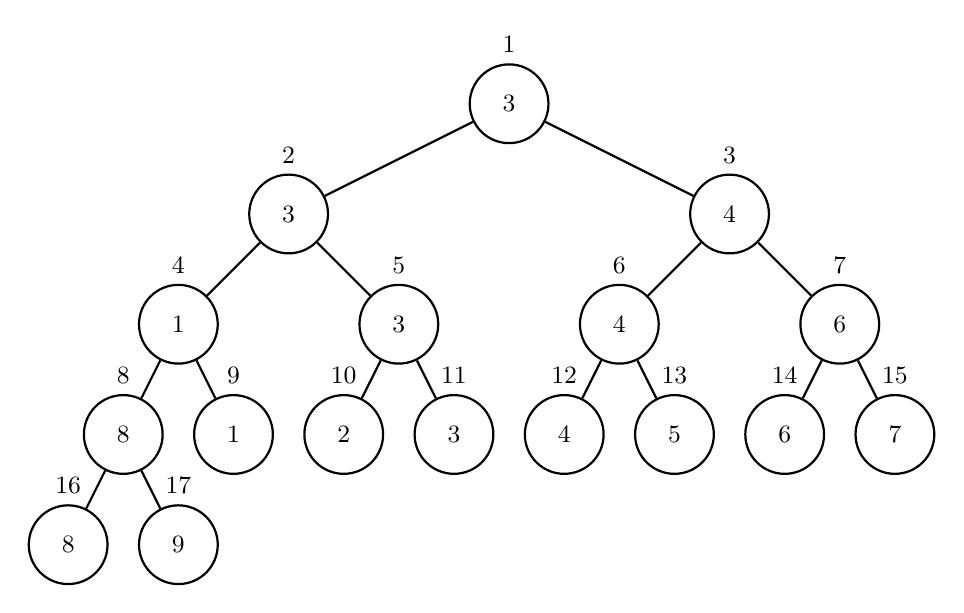
\begin{tikzpicture}[thick, scale=0.7]
        \node[label={1},circle,draw,minimum size=1cm]
        (1) at (0,0) {$3$};
        \node[label={2},circle,draw,minimum size=1cm]
        (2) at (-4,-2) {$3$};
        \node[label={3},circle,draw,minimum size=1cm]
        (3) at (4,-2) {$4$};
        \node[label={4},circle,draw,minimum size=1cm]
        (4) at (-6,-4) {$1$};
        \node[label={5},circle,draw,minimum size=1cm]
        (5) at (-2,-4) {$3$};
        \node[label={6},circle,draw,minimum size=1cm]
        (6) at (2,-4) {$4$};
        \node[label={7},circle,draw,minimum size=1cm]
        (7) at (6,-4) {$6$};
        \node[label={8},circle,draw,minimum size=1cm]
        (8) at (-7,-6) {$8$};
        \node[label={9},circle,draw,minimum size=1cm]
        (9) at (-5,-6) {$1$};
        \node[label={10},circle,draw,minimum size=1cm]
        (10) at (-3,-6) {$2$};
        \node[label={11},circle,draw,minimum size=1cm]
        (11) at (-1,-6) {$3$};
        \node[label={12},circle,draw,minimum size=1cm]
        (12) at (1,-6) {$4$};
        \node[label={13},circle,draw,minimum size=1cm]
        (13) at (3,-6) {$5$};
        \node[label={14},circle,draw,minimum size=1cm]
        (14) at (5,-6) {$6$};
        \node[label={15},circle,draw,minimum size=1cm]
        (15) at (7,-6) {$7$};
        \node[label={16},circle,draw,minimum size=1cm]
        (16) at (-8,-8) {$8$};
        \node[label={17},circle,draw,minimum size=1cm]
        (17) at (-6,-8) {$9$};

        \draw[thick] (1) -- (2);
        \draw[thick] (2) -- (4);
        \draw[thick] (4) -- (8);
        \draw[thick] (4) -- (9);
        \draw[thick] (8) -- (16);
        \draw[thick] (8) -- (17);
        \draw[thick] (2) -- (5);
        \draw[thick] (5) -- (10);
        \draw[thick] (5) -- (11);
        \draw[thick] (1) -- (3);
        \draw[thick] (3) -- (6);
        \draw[thick] (3) -- (7);
        \draw[thick] (6) -- (12);
        \draw[thick] (6) -- (13);
        \draw[thick] (7) -- (14);
        \draw[thick] (7) -- (15);
    \end{tikzpicture}
    \caption[Representação da estrutura torneio]{Torneio com $9$
        elementos em que $3$ é o elemento com valor máximo.}
    \label{fig:torneio:exemplo}
\end{figure}

Queremos dar suporte às seguintes operações:
\begin{itemize}
    \item \textsc{advance}$(t)$ $\rightarrow$ avança o tempo corrente
    para $t$;
    \item \textsc{change}$(j, \vec{v})$ $\rightarrow$ altera a
    velocidade do ponto $j$ para $\vec{v}$;
    \item \textsc{query\textunderscore closest}$()$ $\rightarrow$
    devolve os pontos que formam o par mais próximo no instante
    atual.
\end{itemize}

%!TeX root=./par.tex

\FloatBarrier


\section{Algoritmo estático}\label{sec:algoritmo-estatico}

O algoritmo que será aqui apresentado foi proposto por Basch, Guibas
e Hershberger [\cite{BASCH19991}] e admite uma boa cinetização, usando a ideia de linha
de varredura.

O algoritmo é baseado na ideia de dividir o plano, para cada ponto, em seis cones iguais.
Os cones são delimitados pela reta paralela ao eixo $y$ que passa pelo ponto e pelas retas $x \pm
30^\circ$, isto é, as retas que passam pelo ponto e formam $\pm 30^\circ$ com o eixo $x$ como mostra a
Figura~\ref{fig:parestatico:cones}.

\begin{figure}[H]
    \centering
    \begin{tikzpicture}[thick]
        \draw (0, -3) -- (0, 3) node[anchor=north west] {$y$};
        \draw (-3, 1.7302) -- (3, -1.7302)
        node[anchor=north west] {$x - 30^\circ$};
        \draw (-3, -1.7302) -- (3, 1.7302)
        node[anchor=south west] {$x + 30^\circ$};
        \node[label=250:$p$] (p) at (0, 0) {\textbullet};
    \end{tikzpicture}
    \caption[Exemplo de cones do algoritmo estático]{A reta paralela
    ao eixo $y$ que passa por $p$ e as retas $x \pm 30^\circ$.}
    \label{fig:parestatico:cones}
\end{figure}

Tendo dividido o plano em cones, a ideia é achar o ponto mais próximo de $p$ dentro de cada um
desses cones.
Se assim o fizermos para todos os pontos, um desses pares possui a menor distância entre si e será
um par mais próximo que buscamos.

Se $(p, q)$ formam um par mais próximo, então $(q, p)$ também forma um par mais próximo;
na verdade, são o mesmo par.
Dessa maneira, não precisamos dos seis cones para buscar os pares, somente de três deles.
Para uma varredura da direita para a esquerda, apenas buscaremos os pares mais próximos nos três
cones à direita de p.

Vamos começar analisando o cone cujo eixo central é paralelo ao eixo $x$.
Chamaremos esse cone de \textit{dominância de p} e o representaremos por $\Dom(p)$.
Consideraremos que um ponto em cima da linha $x + 30^\circ$ pertence a $\Dom(p)$ e um ponto em cima de
$x - 30^\circ$ não pertence a $\Dom(p)$ como mostra a Figura~\ref{fig:parestatico:dominancia}.
O mesmo algoritmo poderá ser aplicado aos outros dois cones se rotacionarmos o sistema de
coordenadas~$\pm 60^\circ$.

\begin{figure}[H]
    \centering
    \begin{tikzpicture}[thick, scale=0.8]
        % \draw (0, -3) -- (0, 3) node[anchor=north west] {$y$};
        \draw (0, 0) -- (4, 2.309);
        \draw[dashed] (0, 0) -- (4, -2.309);
        \draw (0, 0) circle (2pt) node[label=250:$p$] {};
        \node[label=0:$q$] (q) at (1, 0) {\textbullet};
        \node[label=250:$r$] (r) at (3, 1.73) {\textbullet};
        \draw (3, -1.73) circle (2pt) node[label=250:$s$] {};
        % \node[label=250:$s$] (s) at (3, -1.73);
    \end{tikzpicture}
    \caption[Exemplo de $\Dom(p)$]{Os pontos $q$ e $r$ pertencem a $\Dom(p)$,
    mas o ponto $s$ não.}
    \label{fig:parestatico:dominancia}
\end{figure}

A Figura~\ref{fig:parestatico:conjuntos}, inspirada em~\cite{BASCH19991}, ilustra cada uma das
definições a seguir.
Definiremos como $\Maxima(p)$ o conjunto dos pontos à direita de $p$ que não pertencem à
dominância de nenhum ponto à direita de $p$.
Isso nos permite definir o conjunto de \textit{candidatos} de $p$ representado por $\Cands(p)$:
$\Cands(p) = \Dom(p) \cap\Maxima(p)$, ou seja, os candidatos de $p$ são aqueles pontos à
direita de $p$ que não pertencem à dominância de nenhum ponto à direita de $p$ e
pertencem à dominância de $p$.
Chamaremos o ponto de $\Maxima$ de menor ordenada que está acima de $\Dom(p)$ de $\up(p)$ e
chamaremos o ponto de $\Maxima$ de maior ordenada que está abaixo de $\Dom(p)$ de $\low(p)$.
Caso não existam tais pontos, $\up(p)$ e $\low(p)$ são \nnull.
Os pontos de $\Maxima$ estritamente entre $\low(p)$ e $\up(p)$ são justamente os de $\Cands(p)$.
Dentre os candidatos de $p$, chamaremos o ponto com menor coordenada $x$ de $\lcand(p)$.

\begin{figure}[H]
    \centering
    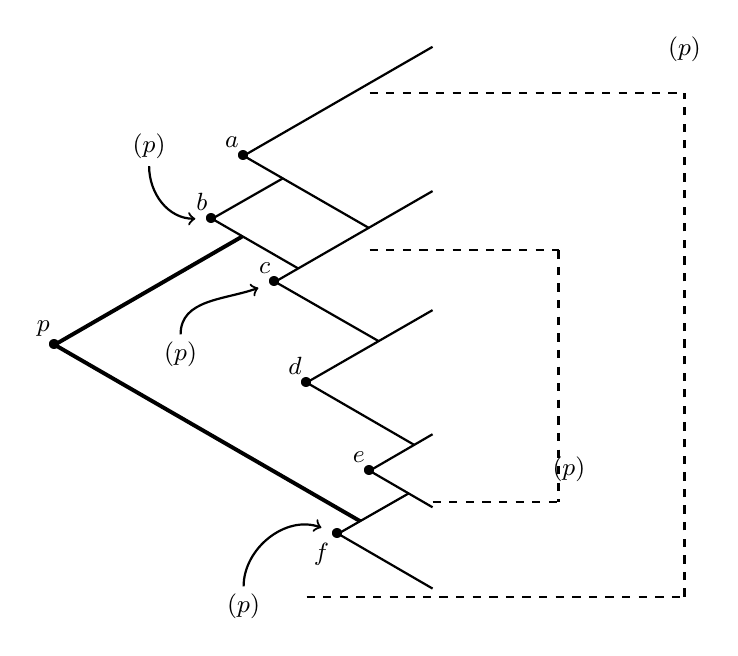
\begin{tikzpicture}[thick, scale=0.8]
        \node[label={[label distance = -3mm]160:$p$}]
        at (0.00, 0.00) {\textbullet};
        \node[label={[label distance = -3mm]160:$a$}]
        (a) at (3.00, 3.00) {\textbullet};
        \node[label={[label distance = -3mm]160:$b$}]
        (b) at (2.50, 2.00) {\textbullet};
        \node[label={[label distance = -3mm]160:$c$}]
        (c) at (3.50, 1.00) {\textbullet};
        \node[label={[label distance = -3mm]160:$d$}]
        at (4.00, -0.60) {\textbullet};
        \node[label={[label distance = -3mm]160:$e$}]
        at (5.00, -2.00) {\textbullet};
        \node[label={[label distance = -3mm]220:$f$}]
        (f) at (4.50, -3.00) {\textbullet};

        % e cone
        \draw (5.00, -2.00) -- (6.00, -2.58);
        \draw (5.00, -2.00) -- (6.00, -1.42);
        % f cone
        \draw (4.50, -3.00) -- (6.00, -3.87);
        \draw (4.50, -3.00) -- (5.62, -2.36);
        % d cone
        \draw (4.00, -0.60) -- (5.71, -1.59);
        \draw (4.00, -0.60) -- (6.00, 0.55);
        % c cone
        \draw (3.50, 1.00) -- (5.14, 0.06);
        \draw (3.50, 1.00) -- (6.00, 2.44);
        % a cone
        \draw (3.00, 3.00) -- (4.98, 1.86);
        \draw (3.00, 3.00) -- (6.00, 4.73);
        % b cone
        \draw (2.50, 2.00) -- (3.87, 1.21);
        \draw (2.50, 2.00) -- (3.62, 2.64);
        % p cone
        \draw[line width = 0.5mm] (0.00, 0.00) -- (4.85, -2.80);
        \draw[line width = 0.5mm] (0.00, 0.00) -- (2.98, 1.72);

        \draw[dashed] (6,-2.5) -- (8, -2.5)
        node[anchor=west, label=90:$\Cands(p)$] {};
        \draw[dashed] (8, 1.5) -- (8, -2.5);
        \draw[dashed] (5,1.5) -- (8, 1.5);

        \draw[dashed] (4, -4) -- (10, -4);
        \draw[dashed] (10, -4) -- (10, 4);
        \draw[dashed] (5, 4) -- (10, 4)
        node[anchor=south, label=$\Maxima(p)$] {};

        \node[label={[label distance = -3mm]270:$\low(p)$}]
        (low) at (3, -4) {};
        \draw[->] (low) edge[out=90,in=160] (f);

        \node[label={[label distance = -3mm]270:$\lcand(p)$}]
        (lc) at (2, 0) {};
        \draw[->] (lc) edge[out=90,in=200] (c);

        \node[label={[label distance = -3mm]90:$\up(p)$}]
        (up) at (1.5, 3) {};
        \draw[->] (up) edge[out=270,in=180] (b);
    \end{tikzpicture}
    \caption[Exemplo dos conjuntos utilizados no algoritmo]{Os pontos
        $c$, $d$ e $e$ pertencem a $\Cands(p)$, e todos os pontos exceto
        $p$ pertencem a $\Maxima(p)$. O ponto $b$ é $\up(p)$ e o ponto
        $f$ é $\low(p)$. O ponto $c$ é $\lcand(p)$.}
    \label{fig:parestatico:conjuntos}
\end{figure}

Consideraremos apenas os pares $(p, \lcand(p))$ como possíveis candidatos a par mais próximo.
Caso, para algum $p$, mais de um ponto atenda à condição de ser $\lcand(p)$ poderemos escolher
qualquer um deles como $\lcand(p)$, pois, em um caso em que há mais de um possível $\lcand(p)$,
esses pontos formarão um par mais próximo entre si do que o par $(p, \lcand(p))$, como por exemplo
na Figura~\ref{fig:parestatico:lcands}.

\begin{figure}[H]
    \centering
    \begin{tikzpicture}[thick, scale=0.8]
        % \draw (0, -3) -- (0, 3) node[anchor=north west] {$y$};
        \draw (0, 0) -- (4, 2.309);
        \draw[dashed] (0, 0) -- (4, -2.309);
        \node[label=250:$p$] (p) at (0, 0) {\textbullet};
        \node[label=0:$q$] (q) at (4, -2) {\textbullet};
        \node[label=250:$r$] (r) at (4, 0) {\textbullet};
        \draw[dotted] (4, -2) -- (4, 0);
        \draw[dotted] (0, 0) -- (r);
        \draw[dotted] (0, 0) -- (q);
    \end{tikzpicture}
    \caption[Exemplo de $\lcand(p)$]{A distância de $r$ até $q$ é menor do que a
    distância de $p$ até $r$ e do que a distância de $p$ até $q$.}
    \label{fig:parestatico:lcands}
\end{figure}

O Algoritmo~\ref{parestatico:horizontal} descreve a sequência de operações a serem feitas para
achar o par mais próximo em alguma das ordens $(-60^\circ, 0^\circ, 60^\circ)$ representadas pelo
ângulo $\theta$, dado em radianos.
Antes da rotina ser chamada, os pontos devem ser ordenados de acordo com a sua coordenada $x$.
Os pontos são então processados da direita para a esquerda.
No algoritmo, $a$ e $b$ são os pontos que representam o par mais próximo.
Se $p$ ou $q$ são nulos, $d(p,q)$ retorna $+\infty$.

A cada iteração do Algoritmo~\ref{parestatico:horizontal}, $\Maxima$ é igual a $\Maxima(p)$.
Na nossa implementação, $\Maxima$ estará armazenado em uma árvore binária de busca, mais
especificamente em uma \textit{splay tree} cuja chave é a coordenada $y$ dos pontos, determinada
de acordo com o valor de $\theta$.
Com isso, podemos buscar por $\up(p)$ e $\low(p)$ em tempo logarítmico, bem como podemos retirar
$\Cands(p)$ de $\Maxima$ em tempo logarítmico, isto é, atualizar $\Maxima$ de maneira que $\Maxima
= \Maxima \setminus \Cands(p)$.

\begin{algorithm}
    \caption[Algoritmo \textsc{closest\_pair} do par mais próximo]{Função \textsc{closest\_pair}$(p, n, \theta)$.}
    \label{alg:par-estatico:horizontal}
    \begin{algorithmic}[1]
        \Function{closest\_pair}{$p, n, \theta$}
            \State \Call{heapsort}{$p, n, \theta$} \Comment{$p[1].x > \cdots > p[n].x$}
            \State $(a,b) \leftarrow (\nnull, \nnull)$
            \State $\Maxima \leftarrow \varnothing$
            \For{$i \leftarrow 1\To n$}
                \State $\Cands \leftarrow \Maxima\cap \Dom(p[i])$
                \State $\Maxima \leftarrow (\Maxima \setminus \Cands) \cup \lk p[i]\rk$
                \State $\lcand \leftarrow \Call{min\_x}{\Cands}$
                \If{$d(p[i], \lcand) < d(a, b)$}
                    \State $(a, b) \leftarrow (p[i], \lcand)$
                \EndIf
            \EndFor
            \State \Return{$(a, b)$}
        \EndFunction
    \end{algorithmic}
\end{algorithm}

Para descrever a implementação do algoritmo, já considerando as versões rotacionadas dele, iremos
antes precisar estabelecer os nomes das variáveis e rotinas auxiliares utilizadas.
São elas:
\begin{enumerate}
    \item $n$: o número de pontos dados;
    \item \textit{point}: um ponto com os seguintes atributos:
    \begin{enumerate}
        \item $x$: coordenada $x$ do ponto;
        \item $y$: coordenada $y$ do ponto.
    \end{enumerate}
    \item \raiz: raiz da splay tree;
    \item \no: objeto que compõe a árvore binária de busca,
    atributos:
    \begin{enumerate}
        \item \esq$:$ aponta para a raiz da subárvore esquerda do nó.
        A subárvore esquerda é composta apenas por pontos que possuem
        \textit{value}~com menor ordenada que a \textit{value}~do nó;
        \item \dir$:$ aponta para a raiz da subárvore direita do nó.
        A subárvore direita é composta apenas por pontos que possuem
        \textit{value}~com ordenada maior ou igual que a \textit{value}~do nó;
        \item \pai$:$ aponta para o nó que é pai deste nó;
        \item \textit{value}$:$ aponta para um ponto.
    \end{enumerate}
    \item \angulo: ângulo de rotação do sistema de coordenadas;
    \item \pontos: vetor de $n$ posições que guarda os pontos;
    \item \textsc{getX}$(p, \angulo) \rightarrow$ retorna a coordenada $x$
    de um ponto $p$ baseada no ângulo de rotação \angulo;
    \item \textsc{getY}$(p, \angulo) \rightarrow$ retorna a coordenada $y$
    de um ponto $p$ baseada no ângulo de rotação \angulo;
    \item \textsc{heapsort}$(\pontos, n, \angulo) \rightarrow$ ordena o vetor \pontos,
    utilizando o algoritmo \textit{heapsort}, de acordo com a coordenada $x$ de cada ponto cujo
    valor é retornado pela rotina \textsc{getX}$(p, \angulo)$.
\end{enumerate}

Para um ponto $(r, \phi)$ em coordenadas polares, $x = r\cdot \cos{(\phi)}$ e $y = r\cdot
\sin{(\phi)}$.

Rotacionar o sistema de coordenadas por $\theta$ é o mesmo que transformar $\phi$ em $\phi -
\theta$, veja a Figura~\ref{fig:parestatico:rotacao}.
Isso significa que agora as novas coordenadas são descritas como:
\begin{align*}
    x^* & = r\cdot \cos{(\phi - \theta)}= r\cdot \cos{(\phi)}\cdot \cos{(\theta)}
    + r\cdot \sin{(\phi)}\cdot \sin{(\theta)} = x\cdot \cos{(\theta)} + y\cdot \sin{(\theta)} \\
    y^* & = r\cdot \sin{(\phi - \theta)} = r\cdot \sin{(\phi)}\cdot \cos{(\theta)}
    - r\cdot \cos{(\phi)}\cdot \sin{(\theta)} = y\cdot \cos{(\theta)} - x\cdot \sin{(\theta)}.
\end{align*}
Os valores $x^*$ e $y^*$ são os valores, respectivamente, retornados por \textsc{getX}$(p,
\angulo)$ e \textsc{getY}$(p, \angulo)$ para $\theta = \angulo$.

\begin{figure}[H]
    \centering
    \begin{tikzpicture}[thick]
        \coordinate (a) at (0, 0);
        \coordinate (b) at (4, 0);
        \coordinate (c) at (2.828, 2.828);
        \coordinate (p) at (1, 2);
        \draw[thick,->] (0,0) -- (4,0)
        node[anchor=north west] {$x$};
        \draw[thick,->] (0,0) -- (0,4)
        node[anchor=south east] {$y$};
        \draw[thick,->, dashed] (0,0) -- (2.828,2.828)
        node[anchor=north west] {$x'$};
        \draw[thick,->, dashed] (0,0) -- (-2.828,2.828)
        node[anchor=south east] {$y'$};
        \pic [draw, angle radius = 0.5cm] {angle = b--a--c};
        \node[anchor=west, label={[label distance = 0mm]180:$\theta$}]
        (angl) at (1, 0.3) {};
        \node[label=90:$p$] at (p) {\textbullet};
        \draw[dashed,->] (a) -- node[above] {$r$} (p);
        \pic [draw, angle radius = 1cm] {angle = b--a--p};
        \node[anchor=west, label={[label distance = -3mm]180:$\phi$}]
        (angp) at (1.2, 0.7) {};
    \end{tikzpicture}
    \caption{O ponto $p$ está numa inclinação de $\phi - \theta$ radianos
    em relação a reta que passa pela origem e por $x'$.}
    \label{fig:parestatico:rotacao}
\end{figure}

A interface da \textit{splay tree} que vai armazenar $\Maxima$, e cuja chave é a coordenada $y$ do
ponto, contará com as seguintes operações, além das usuais \textsc{insert}$(p)$ e
\textsc{splay}$(x)$:
\begin{enumerate}
    \item \textsc{successor}$(p) \rightarrow$ busca pelo nó
    cuja chave é $\up(p)$ na \textit{splay tree}.
    Esse nó corresponde ao sucessor de $p$ na árvore;
    \item \textsc{predecessor}$(p) \rightarrow$ busca pelo nó cuja chave é $low(p)$ na \textit{splay tree}.
    Esse nó corresponde ao predecessor de $p$ na árvore;
    % \item \textsc{splay}$(x) \rightarrow$ dá um \textit{splay} no nó $x$;
    \item \textsc{lcand}$(p) \rightarrow$ calcula $\Cands(p)$, remove da
    \textit{splay tree} e determina $\lcand(p)$, que pode ser \nnull;
    % \item \textsc{clearAll}$() \rightarrow$ remove todos os nós
    % da \textit{splay tree}.
\end{enumerate}

% As operações \textsc{insert}$(p)$, \textsc{splay}$(x)$ e
% \textsc{clearAll}$()$ não possuem nenhuma diferença quanto
% à sua implementação. São operações comuns de uma
% \textit{splay tree}. Portanto, focaremos em explicar as
% operações successor$(p)$, predecessor$(p)$ e lcand$(p)$.

No Algoritmo~\ref{parestatico:successor} e no Algoritmo~\ref{parestatico:predecessor}, a rotina
\textsc{checkLine}$(p, q, \theta)$ retorna se o ponto$q$ está à esquerda, sobre ou à direita da
reta $r$.
A reta $r$ é a reta que passa por $p$ e faz um ângulo de $\theta$ radianos com o eixo $x$.
Para $q$ à esquerda de $r$ o retorno é $1$, para $q$ sobre $r$ o retorno é $0$ e para $q$ à
direita de $r$, o retorno é $-1$.

O Algoritmo~\ref{parestatico:lcand} implementa a função \textsc{lcand}$(p)$.
Sabemos que $\lcand(p)$ é o elemento de $\Cands(p)$ com menor coordenada $x$ e que $\Cands(p)$ é
limitado por $\low(p)$ e $\up(p)$.
A ideia para retirar $\Cands(p)$ da árvore é reorganizá-la de modo que $\low(p)$ seja a raiz e
$\up(p)$ o filho direito da raiz.
Dessa forma $\Cands(p)$ é a subárvore esquerda do filho direito da raiz, veja a
Figura~\ref{fig:parestatico:loweup}.
Nem sempre tal configuração é possível, mas o algoritmo tratará dos casos de borda que são quando
$\low(p)$, ou $\up(p)$, ou ambos, não existem.
A rotina \textsc{split}$(x)$ separa a subárvore de raiz $x$ da \textit{splay tree} e retorna a
raiz dessa nova árvore.
A rotina \textsc{min\_x}$(z)$ retorna o ponto com menor coordenada $x$ da árvore de raiz~$z$.

\begin{figure}
    \centering
    \begin{tikzpicture}[thick]
        \tikzstyle{every node}=[font=\small]
        \node[every node,circle,draw, minimum size=1cm] (low) at (0, 0) {$l$};
        \node[every node,circle,draw, minimum size=1cm] (up) at (2, -2) {$u$};
        \node (esq) at (-2, -2) {$\gamma$};
        \node[every node] (esqesq) at (1, -4) {$\alpha$};
        \node[every node] (esqdir) at (3, -4) {$\beta$};
        \draw (low) -- (up);
        \draw (esqesq) -- (up);
        \draw (esqdir) -- (up);
        \draw (low) -- (esq);
    \end{tikzpicture}
    \caption{Na figura, $l$ é $low(p)$ e $u$ é $up(p)$. A subárvore
    $\alpha$ contém todos os pontos que estão entre $low(p)$ e
    $up(p)$ e, portanto, corresponde ao conjunto $Cands(p)$.}
    \label{fig:parestatico:loweup}
\end{figure}

\begin{algorithm}
    \caption[Algoritmo \textsc{successor} do par mais próximo]{Função \textsc{successor}$(p)$.}
    \label{alg:par-estatico:successor}
    \begin{algorithmic}[1]
        \Function{successor}{$p$}
            \State $x \leftarrow \raiz$ \Comment{raiz da \textit{splay tree}}
            \State $\up \leftarrow \nnull$
            \While{$x \neq \nnull$}
                \State $y \leftarrow x$
                \If{$\Call{checkLine}{p, x.\key, \pi/6}= -1$}
                    \State $x \leftarrow x.\dir$
                \Else
                    \State $\up \leftarrow x$
                    \State $x \leftarrow x.\esq$
                \EndIf
            \EndWhile
            \If{$y \neq \nnull$}
                \Comment{aciona \textsc{splay} no último nó visitado}
                \State \Call{splay}{$y$}
            \EndIf
            \State \Return{$\up$}
        \EndFunction
    \end{algorithmic}
\end{algorithm}

\begin{algorithm}[H]
    \caption[Algoritmo \textsc{predecessor} do par mais próximo]{Função \textsc{predecessor}$(p)$.}
    \label{alg:par-estatico:predecessor}
    \begin{algorithmic}[1]
        \Function{predecessor}{$p$}
            \State $x \leftarrow \raiz$ \Comment{raiz da \textit{splay tree}}
            \State $\low \leftarrow \nnull$
            \While{$x \neq \nnull$}
                \State $y \leftarrow x$
                \If{$\Call{checkLine}{p, x.\key, -\pi/6}\leq 0$}
                    \State $x \leftarrow x.\esq$
                \Else
                    \State $\low \leftarrow x$
                    \State $x \leftarrow x.\dir$
                \EndIf
            \EndWhile
            \If{$y \neq \nnull$}
                \Comment{aciona \textsc{splay} no último nó visitado}
                \State \Call{splay}{$y$}
            \EndIf
            \State \Return{$\low$}
        \EndFunction
    \end{algorithmic}
\end{algorithm}

\begin{algorithm}
    \caption{Função lcand$(p)$.} \label{parestatico:lcand}
\begin{algorithmic}[1]
    \Function{lcand}{$p$}
        \State $r \leftarrow root$
        \State $low \leftarrow \Call{predecessor}{p}$
        \If{$low \neq NULL$}
            \State \Call{splay}{$low$}
            \State $r \leftarrow \Call{split}{low.right}$
        \EndIf
        \State $up \leftarrow \Call{successor}{p}$
        \If{$up \neq NULL$}
            \State $\Call{splay}{up}$
            \State $r \leftarrow \Call{split}{up.left}$
        \EndIf
        \If{$up \neq NULL$ \AND $low \neq NULL$}
            \State $low.right \leftarrow up$
            \State $up.parent \leftarrow low$
        \EndIf
        \State \Return{\Call{min\_x}{$r$}}
    \EndFunction
\end{algorithmic}
\end{algorithm}

O Algoritmo~\ref{alg:par-estatico:closest} implementa a função \textsc{query\_closest} que retorna um
par $(a,b)$ que possui distância mínima em \pontos.

\begin{algorithm}[H]
    \caption{Função \textsc{query\_closest}.} \label{alg:par-estatico:closest}
    \begin{algorithmic}[1]
        \Function{query\_closest}{\null}
            \State $(m,n) \leftarrow (\nnull, \nnull)$
            \State \angulo~$\leftarrow -\frac{\pi}{3}$
            \While{\angulo~$\leq \frac{\pi}{3}$}
                \State \Call{heapsort}{$\pontos, n, \angulo$} \Comment{$\pontos.x[1] > \cdots >
                \pontos.x[n]$}
                \For{$i \leftarrow 1$\To$n$}
                    \State $p \leftarrow $~\pontos$[i]$
                    \State $\lcand \leftarrow $ \Call{lcand}{$p$}
                    \State \Call{insert}{$p$}
                    \If{$d(p, \lcand) < d(a, b)$}
                        \State $(a, b) \leftarrow (p, \lcand)$
                    \EndIf
                \EndFor
                \State \angulo~$\leftarrow$~\angulo~$ + \frac{\pi}{3}$
                \State \Call{clearAll}{\null} \Comment{esvazia a \textit{splay tree}}
            \EndWhile
            \State \Return{$(m,n)$}
        \EndFunction
    \end{algorithmic}
\end{algorithm}


%!TeX root=./par.tex

\FloatBarrier


\section{Algoritmo cinético}\label{sec:algoritmo-cinetico}

Para ``cinetizar'' o algoritmo estático, utilizaremos certificados para assegurar que as nossas
estruturas permanecerão corretas.
Primeiramente, teremos os certificados das três \textit{listas ordenadas cinéticas}, conforme a
Seção~\ref{sec:heap-cinetico}, que guardarão a ordem dos pontos de acordo com os eixos $x$, $x +
60^\circ$ e $x - 60^\circ$.

Para garantir qual, dentre os pares $(p, \lcand(p))$, é o par mais próximo, usaremos um
\textit{torneio cinético com inserção e remoção}, conforme a Seção~\ref{subsec:torneioi:secao},
com respeito ao mínimo em vez de ao máximo.
Temos um total de $3n$ pares, pois consideraremos também os pares $(p, \lcand(p))$ em que
$\lcand(p)$ é nulo e os certificados destes serão $+\infty$.

Também precisaremos manter informação guardada para atualizar com eficiência mudanças provocadas
por trocas na ordem dos pontos em relação a um dos três eixos.
Por exemplo, uma troca na ordem dos pontos pode acarretar numa mudança nos conjuntos $\Cands(p)$ e
$\Cands(q)$.
Mudanças nesses conjuntos ocorrerão quando $q = \up(p)$, $q = \low(p)$ ou $q \in \Cands(p)$.
Portanto, para que consigamos manter $\lcand(p)$ de maneira eficiente, cada ponto terá três árvores
binárias de busca associadas a ele com os conjuntos $\Cands(p)$, $\Hits_{up}(p)$ e $\Hits_{low}(p)
$.
A árvore $\Cands(p)$ guarda os pontos que pertencem ao conjunto $\Cands(p)$ ordenados pela
coordenada $y$.
A árvore $\Hits_{up}(p)$ guarda os pontos $q$ tais que $\up(q) = p$, ordenados pela coordenada $x$.
Similarmente, a árvore $\Hits_{low}(p)$ guarda os pontos $q$ tais que $\low(q) = p$, ordenados
pela coordenada $x$.
Utilizaremos as árvores $\Cands(p)$, $\Hits_{up}(p)$ e $\Hits_{low}(p)$ para cada um dos eixos,
logo, para cada ponto $p$, haverão nove \textit{splay trees} no total.

Cada uma das nove árvores têm sua raiz apontando para o nó $p$, e cada nó das árvores aponta para
o seu nó pai.
Na árvore $\Cands(p)$, cada nó deve apontar para o descendente que contém o ponto mais à esquerda
na ordenação horizontal.
Na nossa implementação, as árvores serão \textit{splay trees}.
Essas estruturas contêm toda a informação necessária para que mantenhamos nossas estruturas
atualizadas e, consequentemente, o par mais próximo do conjunto.

Na implementação do algoritmo, inicialmente inserimos os pontos nas três listas ordenadas.
Uma vez que as listas estejam montadas, percorremos os pontos da direita para a esquerda
preenchendo as estruturas $\Cands(p)$, $\Hits_{up}(p)$ e $\Hits_{low}(p)$ para cada ponto $p$ e
para cada um dos eixos.
Esta etapa é feita da mesma forma que foi apresentada na seção sobre o algoritmo estático, a
Seção~\ref{sec:algoritmo-estatico}.

A medida que as estruturas $\Cands(p)$ são inicializadas, inserimos o par $(p, \lcand(p))$ no
torneio.
Quando todos os pares forem inseridos no torneio, realizamos as partidas e calculamos os
certificados.
O par $(p, q)$ da partida que possuir menor distância é considerado o vencedor.

Todos os certificados são colocados em uma fila de prioridade $Q$.
Os certificados inseridos na fila possuem quatro informações:
\begin{itemize}
    \item $t~\rightarrow$ instante de tempo em que o certificado
    expira.
    É utilizado como chave para a fila de prioridade.
    Desempates são tratados de maneira especial e serão explicados
    mais adiante;
    \item $p~\rightarrow$ um dos pontos envolvidos no evento
    representado pelo certificado.
    Caso seja um certificado de troca na ordenação, $p$ é o ponto mais à direita naquela ordenação;
    \item $q~\rightarrow$ o outro ponto envolvido no evento representado pelo certificado.
    Caso seja um certificado de troca na ordenação, $q$ é o ponto mais à esquerda naquela
    ordenação;
    \item tipo $ \rightarrow$ o tipo de evento que o certificado representa.
    Pode representar uma troca em uma das três ordenações, denominadas por \textit{H} (horizontal =
    $0^\circ$-ordem), \textit{U} (up = $+60^\circ$-ordem) e \textit{D} (down = $-60^\circ$-ordem) ou pode
    representar a vitória do par $(p, q)$ em uma partida do torneio.
\end{itemize}

Vamos agora falar de um evento em que ocorre uma mudança na ordem horizontal.
No primeiro caso, $p$ se encontra à esquerda e abaixo de $q$, veja a
Figura~\ref{fig:parcinetico:eventohorizontalabaixo}.
O caso em que $q$ está à esquerda de $p$ será tratado de maneira parecida.
O Algoritmo~\ref{alg:par-cinetico:eventohorizontal} implementa a sequência de operações referentes a
esse tipo de evento.

\begin{figure}[H]
    \centering
    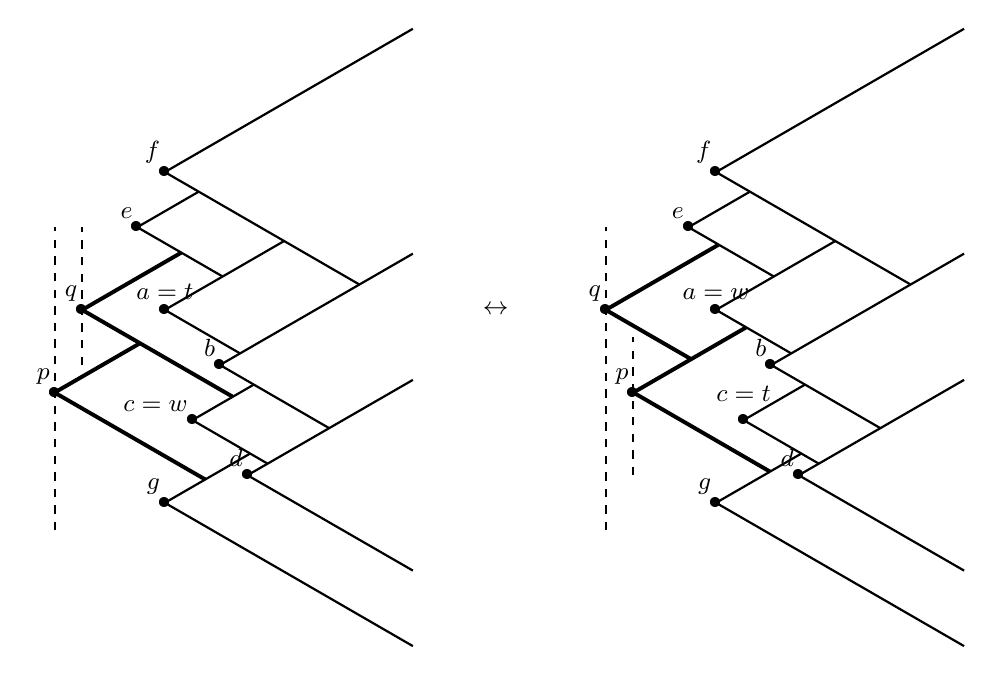
\begin{tikzpicture}[thick, scale=0.35]
        \node[label={[label distance = -3mm]160:$p$}] at
        (2.00, 2.00) {\textbullet};
        \node[label={[label distance = -3mm]160:$q$}] at
        (3.00, 5.00) {\textbullet};
        \node[label={[label distance = -2mm]90:$a = t$}] at
        (6.00, 5.00) {\textbullet};
        \node[label={[label distance = -3mm]160:$b$}] at
        (8.00, 3.00) {\textbullet};
        \node[label={[label distance = -3mm]160:$c = w$}] at
        (7.00, 1.00) {\textbullet};
        \node[label={[label distance = -3mm]160:$d$}] at
        (9.00, -1.00) {\textbullet};
        \node[label={[label distance = -3mm]160:$e$}] at
        (5.00, 8.00) {\textbullet};
        \node[label={[label distance = -3mm]160:$f$}] at
        (6.00, 10.00) {\textbullet};
        \node[label={[label distance = -3mm]160:$g$}] at
        (6.00, -2.00) {\textbullet};
        % d cone
        \draw (9.00, -1.00) -- (15.00, -4.46);
        \draw (9.00, -1.00) -- (15.00, 2.46);
        % b cone
        \draw (8.00, 3.00) -- (11.96, 0.71);
        \draw (8.00, 3.00) -- (15.00, 7.04);
        % c cone
        \draw (7.00, 1.00) -- (9.73, -0.58);
        \draw (7.00, 1.00) -- (9.23, 2.29);
        % f cone
        \draw (6.00, 10.00) -- (13.06, 5.92);
        \draw (6.00, 10.00) -- (15.00, 15.20);
        % g cone
        \draw (6.00, -2.00) -- (15.00, -7.20);
        \draw (6.00, -2.00) -- (9.10, -0.21);
        % a cone
        \draw (6.00, 5.00) -- (8.73, 3.42);
        \draw (6.00, 5.00) -- (10.33, 7.50);
        % e cone
        \draw (5.00, 8.00) -- (8.10, 6.21);
        \draw (5.00, 8.00) -- (7.23, 9.29);
        % q cone
        \draw[line width = 0.5mm] (3.00, 5.00) -- (8.46, 1.85);
        \draw[line width = 0.5mm] (3.00, 5.00) -- (6.60, 7.08);
        % p cone
        \draw[line width = 0.5mm] (2.00, 2.00) -- (7.46, -1.15);
        \draw[line width = 0.5mm] (2.00, 2.00) -- (5.10, 3.79);

        \draw[dashed] (2, -3) -- (2, 8);
        \draw[dashed] (3, 3) -- (3, 8);

        \node at (18, 5) {$ \leftrightarrow$};

        \node[label={[label distance = -3mm]160:$p$}] at
        (23.00, 2.00) {\textbullet};
        \node[label={[label distance = -3mm]160:$q$}] at
        (22.00, 5.00) {\textbullet};
        \node[label={[label distance = -2mm]90:$a = w$}] at
        (26.00, 5.00) {\textbullet};
        \node[label={[label distance = -3mm]160:$b$}] at
        (28.00, 3.00) {\textbullet};
        \node[label={[label distance = -1mm]90:$c = t$}] at
        (27.00, 1.00) {\textbullet};
        \node[label={[label distance = -3mm]160:$d$}] at
        (29.00, -1.00) {\textbullet};
        \node[label={[label distance = -3mm]160:$e$}] at
        (25.00, 8.00) {\textbullet};
        \node[label={[label distance = -3mm]160:$f$}] at
        (26.00, 10.00) {\textbullet};
        \node[label={[label distance = -3mm]160:$g$}] at
        (26.00, -2.00) {\textbullet};
        % d cone
        \draw (29.00, -1.00) -- (35.00, -4.46);
        \draw (29.00, -1.00) -- (35.00, 2.46);
        % b cone
        \draw (28.00, 3.00) -- (31.96, 0.71);
        \draw (28.00, 3.00) -- (35.00, 7.04);
        % c cone
        \draw (27.00, 1.00) -- (29.73, -0.58);
        \draw (27.00, 1.00) -- (29.23, 2.29);
        % f cone
        \draw (26.00, 10.00) -- (33.06, 5.92);
        \draw (26.00, 10.00) -- (35.00, 15.20);
        % g cone
        \draw (26.00, -2.00) -- (35.00, -7.20);
        \draw (26.00, -2.00) -- (29.10, -0.21);
        % a cone
        \draw (26.00, 5.00) -- (28.73, 3.42);
        \draw (26.00, 5.00) -- (30.33, 7.50);
        % e cone
        \draw (25.00, 8.00) -- (28.10, 6.21);
        \draw (25.00, 8.00) -- (27.23, 9.29);
        % p cone
        \draw[line width = 0.5mm] (23.00, 2.00) -- (27.96, -0.87);
        \draw[line width = 0.5mm] (23.00, 2.00) -- (27.10, 4.37);
        % q cone
        \draw[line width = 0.5mm] (22.00, 5.00) -- (25.10, 3.21);
        \draw[line width = 0.5mm] (22.00, 5.00) -- (26.10, 7.37);

        \draw[dashed] (22, -3) -- (22, 8);
        \draw[dashed] (23, -1) -- (23, 4);
    \end{tikzpicture}
    \caption[Exemplo de evento \textsc{horizontal}]{Da esquerda para a direita, o caso em que
    $p$ está em $\Hits_{up}(q)$.
    Da direita para a esquerda, o caso em que $q$ está em $\Hits_{low}(p)$.}
    \label{fig:parcinetico:eventohorizontal}
\end{figure}

Se $p$ está em $\Hits_{up}(q)$, como demonstrado na
Figura~\ref{fig:parcinetico:eventohorizontalabaixo}, então parte de $\Cands(q)$ terá de passar
para $\Cands(p)$.
Para tal, buscamos pelo novo $t = \up(p)$ em $\Cands(q)$ e chamamos a rotina \textit{splay} no
nó que contém $t$.
Após o \textit{splay}, chamamos um \textit{split} na subárvore esquerda desse nó e a unimos a
$\Cands(p)$.
Se $t$ não for encontrado em $\Cands(q)$, então $t = \up(q)$ e todos os pontos de $\Cands(q)$
devem ser transferidos para $\Cands(p)$.
Não podemos esquecer de remover $p$ de $\Hits_{up}(q)$ e adicioná-lo a $\Hits_{up}(t)$, além de
remover $q$ de $\Hits_{low}(w)$ e adicioná-lo a $\Hits_{low}(p)$.
Se $p$ não está em $\Hits_{up}(q)$, então não haverão mudanças, veja a
Figura~\ref{fig:parcinetico:eventohorizontalabaixosemmudancas}.

\begin{figure}[H]
    \centering
    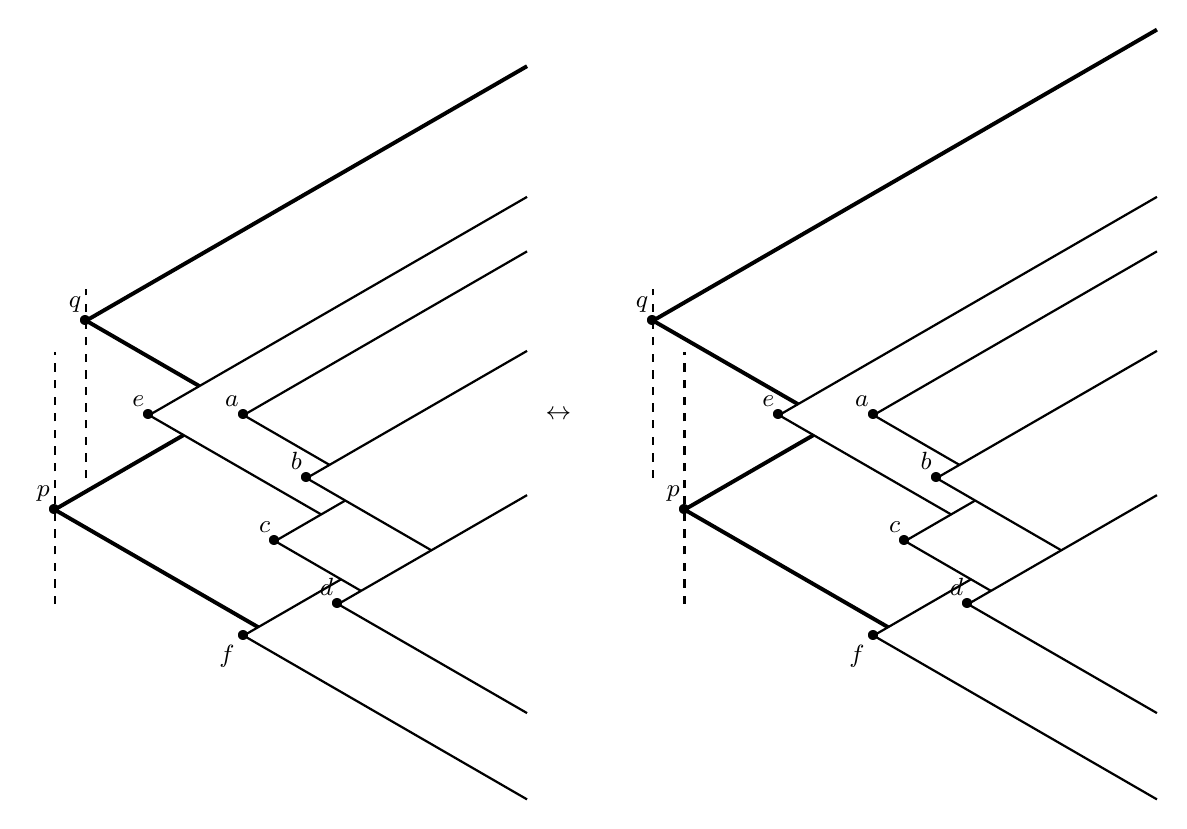
\begin{tikzpicture}[thick, scale=0.4]
        \node[label={[label distance = -3mm]160:$p$}] at
        (0.00, 2.00) {\textbullet};
        \node[label={[label distance = -3mm]160:$e$}] at
        (3.00, 5.00) {\textbullet};
        \node[label={[label distance = -3mm]160:$a$}] at
        (6.00, 5.00) {\textbullet};
        \node[label={[label distance = -3mm]160:$b$}] at
        (8.00, 3.00) {\textbullet};
        \node[label={[label distance = -3mm]160:$c$}] at
        (7.00, 1.00) {\textbullet};
        \node[label={[label distance = -3mm]160:$d$}] at
        (9.00, -1.00) {\textbullet};
        \node[label={[label distance = -3mm]160:$q$}] at
        (1.00, 8.00) {\textbullet};
        \node[label={[label distance = -3mm]220:$f$}] at
        (6.00, -2.00) {\textbullet};

        % d cone
        \draw (9.00, -1.00) -- (15.00, -4.46);
        \draw (9.00, -1.00) -- (15.00, 2.46);
        % b cone
        \draw (8.00, 3.00) -- (11.96, 0.71);
        \draw (8.00, 3.00) -- (15.00, 7.04);
        % c cone
        \draw (7.00, 1.00) -- (9.73, -0.58);
        \draw (7.00, 1.00) -- (9.23, 2.29);
        % f cone
        \draw (6.00, -2.00) -- (15.00, -7.20);
        \draw (6.00, -2.00) -- (9.10, -0.21);
        % a cone
        \draw (6.00, 5.00) -- (8.73, 3.42);
        \draw (6.00, 5.00) -- (15.00, 10.20);
        % e cone
        \draw (3.00, 5.00) -- (8.46, 1.85);
        \draw (3.00, 5.00) -- (15.00, 11.93);
        % q cone
        \draw[line width = 0.5mm] (1.00, 8.00) -- (4.60, 5.92);
        \draw[line width = 0.5mm] (1.00, 8.00) -- (15.00, 16.08);
        % p cone
        \draw[line width = 0.5mm] (0.00, 2.00) -- (6.46, -1.73);
        \draw[line width = 0.5mm] (0.00, 2.00) -- (4.10, 4.37);

        \draw[dashed] (0, -1) -- (0, 7);
        \draw[dashed] (1, 3) -- (1, 9);
        \draw[dashed] (20, -1) -- (20, 7);
        \draw[dashed] (19, 3) -- (19, 9);

        \node at (16, 5) {$ \leftrightarrow$};

        \node[label={[label distance = -3mm]160:$p$}] at
        (20.00, 2.00) {\textbullet};
        \node[label={[label distance = -3mm]160:$e$}] at
        (23.00, 5.00) {\textbullet};
        \node[label={[label distance = -3mm]160:$a$}] at
        (26.00, 5.00) {\textbullet};
        \node[label={[label distance = -3mm]160:$b$}] at
        (28.00, 3.00) {\textbullet};
        \node[label={[label distance = -3mm]160:$c$}] at
        (27.00, 1.00) {\textbullet};
        \node[label={[label distance = -3mm]160:$d$}] at
        (29.00, -1.00) {\textbullet};
        \node[label={[label distance = -3mm]160:$q$}] at
        (19.00, 8.00) {\textbullet};
        \node[label={[label distance = -3mm]220:$f$}] at
        (26.00, -2.00) {\textbullet};

        % d cone
        \draw (29.00, -1.00) -- (35.00, -4.46);
        \draw (29.00, -1.00) -- (35.00, 2.46);
        % b cone
        \draw (28.00, 3.00) -- (31.96, 0.71);
        \draw (28.00, 3.00) -- (35.00, 7.04);
        % c cone
        \draw (27.00, 1.00) -- (29.73, -0.58);
        \draw (27.00, 1.00) -- (29.23, 2.29);
        % f cone
        \draw (26.00, -2.00) -- (35.00, -7.20);
        \draw (26.00, -2.00) -- (29.10, -0.21);
        % a cone
        \draw (26.00, 5.00) -- (28.73, 3.42);
        \draw (26.00, 5.00) -- (35.00, 10.20);
        % e cone
        \draw (23.00, 5.00) -- (28.46, 1.85);
        \draw (23.00, 5.00) -- (35.00, 11.93);
        % p cone
        \draw[line width = 0.5mm] (20.00, 2.00) -- (26.46, -1.73);
        \draw[line width = 0.5mm] (20.00, 2.00) -- (24.10, 4.37);
        % q cone
        \draw[line width = 0.5mm] (19.00, 8.00) -- (23.60, 5.35);
        \draw[line width = 0.5mm] (19.00, 8.00) -- (35.00, 17.24);
    \end{tikzpicture}
    \caption{Se $p$ não está em $\Hits_{up}(q)$, ou se
        $q$ não está em $\Hits_{low}(p)$, nada acontece.}
    \label{fig:parcinetico:eventohorizontalabaixosemmudancas}
\end{figure}

Similarmente, se $q$ está em $\Hits_{low}(p)$, como demonstrado na
Figura~\ref{fig:parcinetico:eventohorizontalabaixo}, parte de $\Cands(p)$ passará a $\Cands(q)$
.
Para realizar tal operação, buscamos pelo novo $t = low(q)$ em $\Cands(p)$, damos um \textit{splay}
no nó que contém $t$, separamos a subárvore direita desse nó e a unimos a $\Cands(q)$.
Se $t$ não for encontrado em $\Cands(p)$, então $t = low(p)$ e todos os pontos de $\Cands(p)$ devem
ser passados para $\Cands(q)$.
Devemos também remover $q$ de $Hits_{low}(p)$ e inseri-lo em $Hits_{low}(t)$, além de remover $p$
de $Hits_{up}(w)$ e adicioná-lo a $Hits_{up}(q)$.
Se $q$ não está em $Hits_{low}(p)$, então não haverão mudanças, veja a
Figura~\ref{fig:parcinetico:eventohorizontalabaixosemmudancas}.

\begin{algorithm}[H]
    \caption[Algoritmo \textsc{horizontalEvent} do par mais próximo cinético]{Função \textsc{horizontalEvent}.}
    \label{alg:par-cinetico:eventohorizontal}
    \begin{algorithmic}[1]
        \Function{horizontalEvent}{$p,q, dir$}
            \If{$q = \Call{owner}{p.\hitsup(dir)}$}
                \State \Call{horizontalEventLeft}{$p,q, dir$}
            \Else
                \If{$p = \Call{owner}{q.\hitslow(p, dir)}$}
                    \State \Call{horizontalEventRight}{$p,q, dir$}
                \EndIf
            \EndIf
            \State $v \leftarrow \Call{owner}{p.cands(dir)}$
            \State $v' \leftarrow \Call{owner}{q.cands(dir)}$
            \If{$v = v'$}
                \State \Call{updateLcand}{$v, dir$}
            \EndIf
        \EndFunction
    \end{algorithmic}
\end{algorithm}

No caso de um evento em que ocorre uma mudança na $60^\circ$-ordem, que é a ordem dos pontos
projetados no eixo $x + 60^\circ$, vamos assumir que $p$ é o ponto que está à esquerda e acima de $q$.
O evento pode provocar a entrada ou saída do ponto $q$ de $\Cands(p)$, veja a
Figura~\ref{fig:parcinetico:eventoup}.
O Algoritmo~\ref{alg:par-cinetico:eventoup} implementa a sequência de operações referentes a este
evento.

Se $p$ está em $\Hits_{low}(q)$, ou seja, $q$ está entrando em $\Dom(p)$ como demonstrado na
Figura~\ref{fig:parcinetico:eventoup} da esquerda para direita, então a troca na $60^\circ$-ordem
afetará o ponto $v$ tal que $q$ está em $\Cands(v)$.
Achamos esse ponto subindo em $\Cands(v)$, a partir do nó que contém $q$, até a raiz que aponta
para $v$.
Devemos então remover $q$ de $\Cands(v)$ e inseri-lo em $\Cands(p)$.
A mudança também afetará todos os pontos que estão à esquerda de $p$ e estão em $\Hits_{up}(q)$.
Para achar esses pontos, buscamos o ponto $t$ em $\Hits_{up}(q)$ mais à esquerda que está à
direita de $p$.
Chamamos \textit{splay} para o nó que contém $t$ e chamamos \textit{split} para a subárvore
esquerda desse nó e juntamos essa árvore em $\Hits_{up}(p)$, pois são todos os pontos à esquerda
de $p$ que tinham $q$ como $\up$ e agora seu novo $\up$ é $p$.
Se esse ponto $t$ não existe, todos os pontos de $\Hits_{up}(q)$ devem ser transferidos para
$\Hits_{up}(p)$, veja a Figura~\ref{fig:parcinetico:eventouptnaoexiste}, e buscamos pelo ponto $t$
tal que $q$ está em $\Hits_{low}(t)$.
Por fim, removemos o ponto $p$ de $\Hits_{low}(q)$ e o inserimos em $\Hits_{low}(t)$.
Se $p$ não está em $\Hits_{low}(q)$ não haverão mudanças.

Se $q$ está em $\Cands(p)$, ou seja, $q$ está saindo de $\Dom(p)$ como demonstrado na
Figura~\ref{fig:parcinetico:eventoup} da direita para a esquerda, então a troca afetará o ponto $t$
tal que $p$ está em $\Hits_{low}(t)$.
Se o ponto $t$ existe, removemos $p$ de $\Hits_{low}(t)$.
Devemos agora inserir $p$ em $\Hits_{low}(q)$, já que $q$ é o novo $\low(p)$.
A mudança também afetará os pontos de $\Hits_{up}(p)$ que agora deverão estar em $\Hits_{up}(q)$.
Para achar esses pontos, buscamos pelo ponto $v$ em $\Hits_{up}(p)$ mais à direita que não deveria
estar em $\Hits_{up}(q)$, chamamos \textit{splay} para o nó que contém $v$ e um \textit{split}
para sua subárvore direita.
Essa nova árvore deve ser incorporada a $\Hits_{up}(q)$.
Se tal ponto $v$ não existe, todos os nós de $\Hits_{up}(p)$ devem ser passados para $\Hits_{up}
(q)$.
Por fim, devemos achar o novo ponto $u$ tal que $q$ deve estar em $\Cands(u)$.
Se o ponto $v$ descrito anteriormente existe, então $u = v$.
Se $v$ não existe, então $u$ é o ponto tal que $p$ está em $\Cands(u)$.
Dessa forma, retiramos $q$ de $\Cands(p)$ e o inserimos em $\Cands(u)$.
Se $q$ não está em $\Cands(p)$, não haverão mudanças.

\begin{algorithm}[H]
    \caption{Função \textsc{upEvent}.}
    \label{alg:par-cinetico:eventoup}
    \begin{algorithmic}[1]
        \Function{upEvent}{$p, q, dir$}
            \If{$q = \Call{owner}{p.hitsLow(dir)}$}
                \State \Call{upEventLeft}{$p, q, dir$}
            \Else
                \If{$p = \Call{owner}{q.cands(dir)}$}
                    \State \Call{upEventRight}{$p, q, dir$}
                \EndIf
            \EndIf
        \EndFunction
    \end{algorithmic}
\end{algorithm}

\begin{algorithm}[H]
    \caption{Função \textsc{upEvent}.}
    \label{alg:par-cinetico:eventoup}
    \begin{algorithmic}[1]
        \Function{upEvent}{$p, q, dir$}
            \If{$q = \Call{owner}{p.hitsLow(dir)}$}
                \State \Call{upEventLeft}{$p, q, dir$}
            \Else
                \If{$p = \Call{owner}{q.cands(dir)}$}
                    \State \Call{upEventRight}{$p, q, dir$}
                \EndIf
            \EndIf
        \EndFunction
    \end{algorithmic}
\end{algorithm}

\begin{figure}[h]
    \centering
    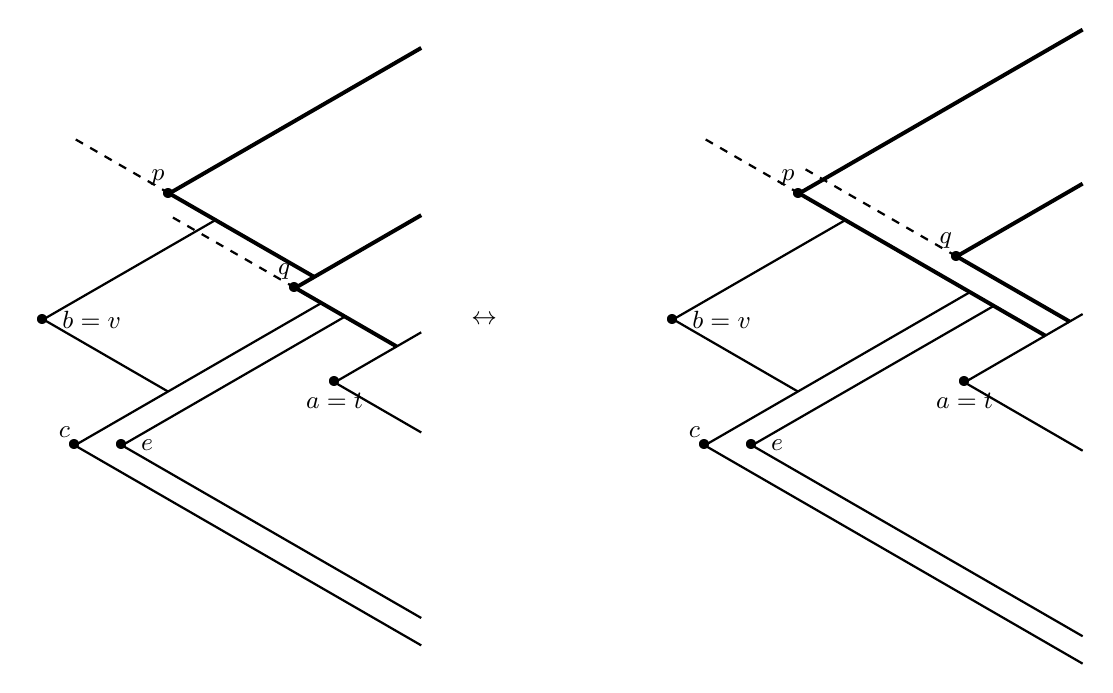
\begin{tikzpicture}[thick, scale=0.4]
        \node[label={[label distance = -3mm]160:$p$}] at
        (2.00, 4.00) {\textbullet};
        \node[label={[label distance = -3mm]160:$q$}] at
        (6.00, 1.00) {\textbullet};
        \node[label={[label distance = -2mm]270:$a = t$}] at
        (7.25, -2.00) {\textbullet};
        \node[label={[label distance = -3mm]160:$c$}] at
        (-1.00, -4.00) {\textbullet};
        \node[label={[label distance = -1mm]0:$b = v$}] at
        (-2.00, 0.00) {\textbullet};
        \node[label={[label distance = -1mm]0:$e$}] at
        (0.50, -4.00) {\textbullet};

        % a cone
        \draw (7.25, -2.00) -- (10.00, -3.59);
        \draw (7.25, -2.00) -- (10.00, -0.41);
        % q cone
        \draw[line width = 0.5mm] (6.00, 1.00) -- (9.22, -0.86);
        \draw[line width = 0.5mm] (6.00, 1.00) -- (10.00, 3.31);
        % p cone
        \draw[line width = 0.5mm] (2.00, 4.00) -- (6.60, 1.35);
        \draw[line width = 0.5mm] (2.00, 4.00) -- (10.00, 8.62);
        % e cone
        \draw (0.50, -4.00) -- (10.00, -9.48);
        \draw (0.50, -4.00) -- (7.58, 0.09);
        % c cone
        \draw (-1.00, -4.00) -- (10.00, -10.35);
        \draw (-1.00, -4.00) -- (6.83, 0.52);
        % b cone
        \draw (-2.00, 0.00) -- (1.96, -2.29);
        \draw (-2.00, 0.00) -- (3.46, 3.15);


        \draw[dashed] (2.00, 4.00) -- (-1.00, 5.73);
        \draw[dashed] (6.00, 1.00) -- (2.00, 3.30);
        \node at (12, 0) {$ \leftrightarrow$};

        \node[label={[label distance = -3mm]160:$p$}] at
        (22.00, 4.00) {\textbullet};
        \node[label={[label distance = -3mm]160:$q$}] at
        (27.00, 2.00) {\textbullet};
        \node[label={[label distance = -2mm]270:$a = t$}] at
        (27.25, -2.00) {\textbullet};
        \node[label={[label distance = -3mm]160:$c$}] at
        (19.00, -4.00) {\textbullet};
        \node[label={[label distance = -1mm]0:$b = v$}] at
        (18.00, 0.00) {\textbullet};
        \node[label={[label distance = -1mm]0:$e$}] at
        (20.50, -4.00) {\textbullet};

        % a cone
        \draw (27.25, -2.00) -- (31.00, -4.17);
        \draw (27.25, -2.00) -- (31.00, 0.17);
        % q cone
        \draw[line width = 0.5mm] (27.00, 2.00) -- (30.59, -0.07);
        \draw[line width = 0.5mm] (27.00, 2.00) -- (31.00, 4.31);
        % p cone
        \draw[line width = 0.5mm] (22.00, 4.00) -- (29.82, -0.52);
        \draw[line width = 0.5mm] (22.00, 4.00) -- (31.00, 9.20);
        % e cone
        \draw (20.50, -4.00) -- (31.00, -10.06);
        \draw (20.50, -4.00) -- (28.18, 0.43);
        % c cone
        \draw (19.00, -4.00) -- (31.00, -10.93);
        \draw (19.00, -4.00) -- (27.43, 0.87);
        % b cone
        \draw (18.00, 0.00) -- (21.96, -2.29);
        \draw (18.00, 0.00) -- (23.46, 3.15);

        \draw[dashed] (22.00, 4.00) -- (19.00, 5.73);
        \draw[dashed] (27.00, 2.00) -- (22.00, 4.88);
    \end{tikzpicture}
    \caption{Da esquerda para a direita,
        todos os pontos de $\Hits_{up}(q)$
        são transferidos para $\Hits_{up}(p)$
        e $p$, que está em $\Hits_{low}(q)$,
        é transferido para $\Hits_{low}(t)$.
        Da direita para a esquerda, os pontos
        em $\Hits_{up}(p)$ são transferidos
        para $\Hits_{up}(q)$ e $p$, que está
        em $\Hits_{low}(t)$, é transferido
        para $\Hits_{low}(q)$.}
    \label{fig:parcinetico:eventouptnaoexiste}
\end{figure}

Um evento em que ocorre uma mudança na $-60^\circ$-ordem, a ordem dos pontos projetados no eixo $x -
60^\circ$, é simétrico a um evento na $60^\circ$-ordem.
Os pontos envolvidos no evento serão $p$e $q$ e vamos assumir que $p$ é o ponto mais à esquerda e
abaixo de $q$.
O evento pode provocar a entrada ou saída do ponto $q$ de $\Cands(p)$, veja a
Figura~\ref{fig:parcinetico:eventodown}.
O Algoritmo~\ref{fig:parcinetico:eventodown} implementa a sequência de operações referentes a esse
evento.

Se $p$ está em $\Hits_{up}(q)$ ($q$ está entrando em $Dom(p)$), como demonstrado na
Figura~\ref{fig:parcinetico:eventodown}, então a troca na $-60^\circ$-ordem afetará o ponto $v$ tal
que $q$ está em $\Cands(v)$.
Achamos esse ponto subindo em $\Cands(v)$, a partir do nó que contém $q$, até a raiz que aponta
para~$v$.
Devemos então remover $q$ de $\Cands(v)$ e inseri-lo em $\Cands(p)$.
A mudança também afetará todos os pontos que estão à esquerda de $p$ e estão em $\Hits_{low}(q)$.
Para achar esses pontos buscamos o ponto $t$ em $\Hits_{low}(q)$ mais à esquerda que está a
direita de $p$.
Chamamos \textit{splay} para o nó que contém $t$ e \textit{split} para a nova subárvore esquerda
desse nó e juntamos essa árvore em $\Hits_{low}(p)$, pois são todos pontos à esquerda de $p$ que
tinham $q$ como $low$ e agora seu novo $low$ é $p$.
Se esse ponto $t$ não existe, veja a Figura~\ref{fig:parcinetico:eventodowntnaoexiste}, então
buscamos pelo ponto $t$ tal que $q$ está em $\Hits_{up}(t)$.
Por fim, removemos o ponto $p$ de $\Hits_{up}(q)$ e o inserimos em $\Hits_{up}(t)$.
Se $p$ não está em $\Hits_{up}(q)$ não haverão mudanças.

Se $q$ está em $\Cands(p)$ ($q$ está saindo de $Dom(p)$), como demonstrado na
Figura~\ref{fig:parcinetico:eventodown}, então a troca afetará o ponto $t$ tal que $p$ está em
$\Hits_{up}(t)$.
Se o ponto $t$ existe, removemos $p$ de $\Hits_{up}(t)$.
Devemos agora inserir $p$ em $\Hits_{up}(q)$, já que $q$ é o novo $up(p)$.
A mudança também afetará os pontos de $\Hits_{low}(p)$ que agora atingem $Dom(q)$.
Para achar esses pontos, buscamos pelo ponto $v$ em $\Hits_{low}(p)$ mais à direita que não atinge
$Dom(q)$, chamamos \textit{splay} para o nó que contém $v$ e um \textit{split} para sua subárvore
direita.
Essa nova árvore deve ser incorporada a $\Hits_{low}(q)$.
Se tal ponto $v$ não existe, todos os nós de $\Hits_{low}(p)$ devem ser passados para $\Hits_{low}
(q)$.
Por fim, devemos achar o novo ponto~$u$ tal que $q$ deve estar em $\Cands(u)$.
Se o ponto $v$ descrito anteriormente existe, então~$u = v$.
Se $v$ não existe, então $u$ é o ponto tal que $p$ está em $\Cands(u)$.
Dessa forma, retiramos $q$ de $\Cands(p)$ e o inserimos em $\Cands(u)$.
Se $q$ não está em $\Cands(p)$, não haverão mudanças.

\begin{figure}[h]
    \centering
    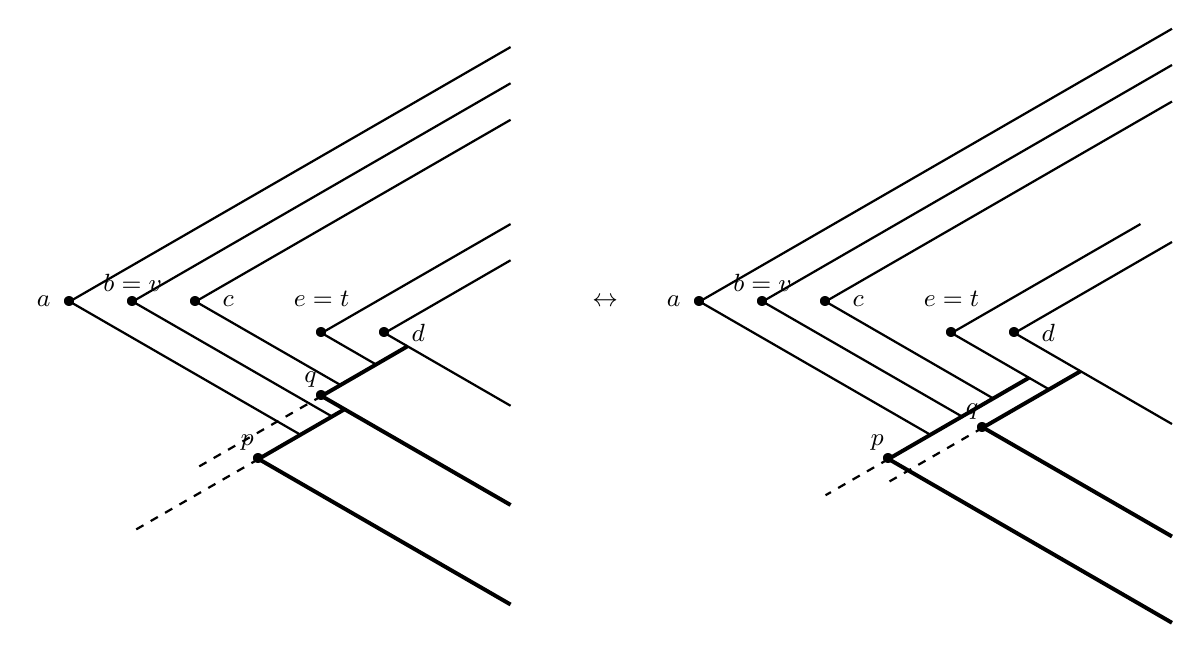
\begin{tikzpicture}[thick, scale=0.4]
        \node[label={[label distance = -3mm]160:$p$}] at
            (6.00, 0.00) {\textbullet};
        \node[label={[label distance = -3mm]160:$q$}] at
            (8.00, 2.00) {\textbullet};
        \node[label={[label distance = -1mm]180:$a$}] at
            (0.00, 5.00) {\textbullet};
        \node[label={[label distance = -2mm]90:$b = v$}] at
            (2.00, 5.00) {\textbullet};
        \node[label={[label distance = 0mm]0:$c$}] at
            (4.00, 5.00) {\textbullet};
        \node[label={[label distance = 0mm]0:$d$}] at
            (10.00, 4.00) {\textbullet};
        \node[label={[label distance = 0mm]90:$e = t$}] at
            (8.00, 4.00) {\textbullet};

        % d cone
        \draw (10.00, 4.00) -- (14.00, 1.69);
        \draw (10.00, 4.00) -- (14.00, 6.31);
        % q cone
        \draw[dashed] (8.00, 2.00) -- (4.00, -0.30);
        \draw[line width = 0.5mm] (8.00, 2.00) -- (14.00, -1.46);
        \draw[line width = 0.5mm] (8.00, 2.00) -- (10.73, 3.58);
        % e cone
        \draw (8.00, 4.00) -- (9.73, 3.00);
        \draw (8.00, 4.00) -- (14.00, 7.46);
        % p cone
        \draw[dashed] (6.00, 0.00) -- (2.00, -2.30);
        \draw[line width = 0.5mm] (6.00, 0.00) -- (14.00, -4.62);
        \draw[line width = 0.5mm] (6.00, 0.00) -- (8.73, 1.58);
        % c cone
        \draw (4.00, 5.00) -- (8.60, 2.35);
        \draw (4.00, 5.00) -- (14.00, 10.77);
        % b cone
        \draw (2.00, 5.00) -- (8.33, 1.35);
        \draw (2.00, 5.00) -- (14.00, 11.93);
        % a cone
        \draw (0.00, 5.00) -- (7.33, 0.77);
        \draw (0.00, 5.00) -- (14.00, 13.08);

        \node at (17, 5) {$ \leftrightarrow$};

        \node[label={[label distance = -3mm]160:$p$}] at
            (26.00, 0.00) {\textbullet};
        \node[label={[label distance = -3mm]160:$q$}] at
            (29.00, 1.00) {\textbullet};
        \node[label={[label distance = -1mm]180:$a$}] at
            (20.00, 5.00) {\textbullet};
        \node[label={[label distance = -2mm]90:$b = v$}] at
            (22.00, 5.00) {\textbullet};
        \node[label={[label distance = 0mm]0:$c$}] at
            (24.00, 5.00) {\textbullet};
        \node[label={[label distance = 0mm]0:$d$}] at
            (30.00, 4.00) {\textbullet};
        \node[label={[label distance = 0mm]90:$e = t$}] at
            (28.00, 4.00) {\textbullet};

        % d cone
        \draw (30.00, 4.00) -- (35.00, 1.11);
        \draw (30.00, 4.00) -- (35.00, 6.89);
        % q cone
        \draw[dashed] (29.00, 1.00) -- (26.00, -0.73);
        \draw[line width = 0.5mm] (29.00, 1.00) -- (35.00, -2.46);
        \draw[line width = 0.5mm] (29.00, 1.00) -- (32.10, 2.79);
        % e cone
        \draw (28.00, 4.00) -- (31.10, 2.21);
        \draw (28.00, 4.00) -- (34.00, 7.46);
        % p cone
        \draw[dashed] (26.00, 0.00) -- (24.00, -1.15);
        \draw[line width = 0.5mm] (26.00, 0.00) -- (35.00, -5.20);
        \draw[line width = 0.5mm] (26.00, 0.00) -- (30.46, 2.58);
        % c cone
        \draw (24.00, 5.00) -- (29.33, 1.92);
        \draw (24.00, 5.00) -- (35.00, 11.35);
        % b cone
        \draw (22.00, 5.00) -- (28.33, 1.35);
        \draw (22.00, 5.00) -- (35.00, 12.51);
        % a cone
        \draw (20.00, 5.00) -- (27.33, 0.77);
        \draw (20.00, 5.00) -- (35.00, 13.66);
    \end{tikzpicture}
    \caption{Da esquerda para direita, o caso em que
    $p$ está em $\Hits_{up}(q)$, ou seja, $q$ está
    entrando em $\Dom(p)$. Da direita para esquerda,
    o caso em que $q$ está em $\Cands(p)$, saindo
    de $\Dom(p)$.}
    \label{fig:parcinetico:eventodown}
\end{figure}

\begin{figure}[h]
    \centering
    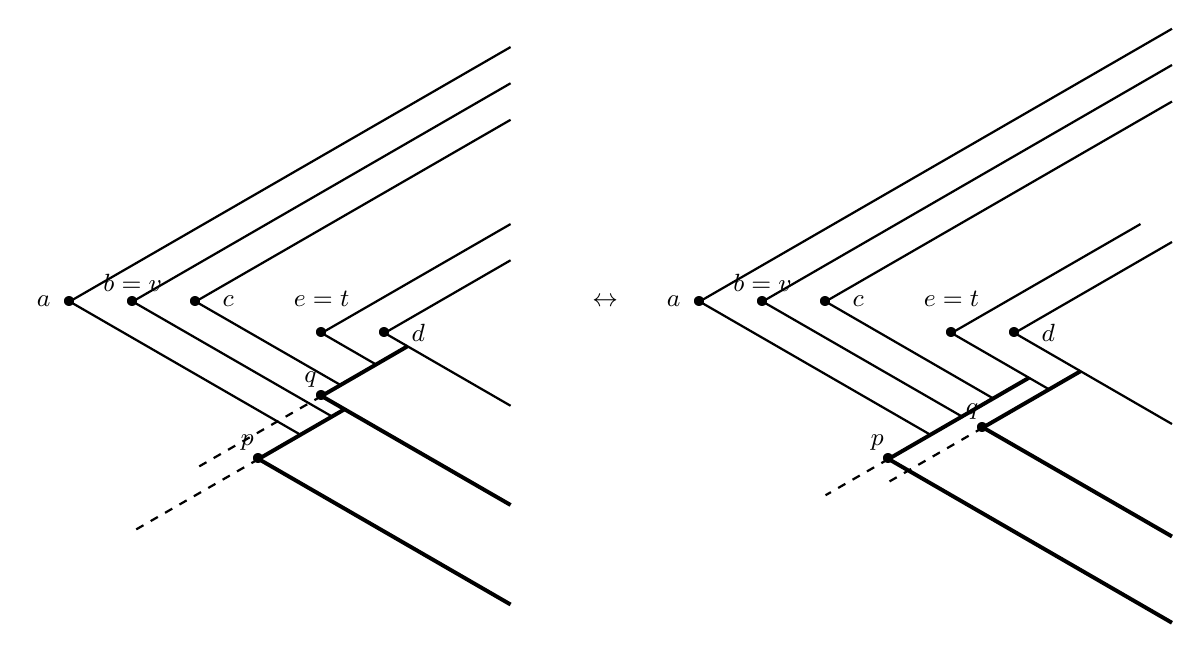
\begin{tikzpicture}[thick, scale=0.4]
        \node[label={[label distance = -3mm]160:$p$}] at
            (6.00, 0.00) {\textbullet};
        \node[label={[label distance = -3mm]160:$q$}] at
            (8.00, 2.00) {\textbullet};
        \node[label={[label distance = -1mm]180:$a$}] at
            (0.00, 5.00) {\textbullet};
        \node[label={[label distance = -2mm]90:$b = v$}] at
            (2.00, 5.00) {\textbullet};
        \node[label={[label distance = 0mm]0:$c$}] at
            (4.00, 5.00) {\textbullet};
        \node[label={[label distance = 0mm]0:$d$}] at
            (10.00, 4.00) {\textbullet};
        \node[label={[label distance = 0mm]90:$e = t$}] at
            (8.00, 4.00) {\textbullet};

        % d cone
        \draw (10.00, 4.00) -- (14.00, 1.69);
        \draw (10.00, 4.00) -- (14.00, 6.31);
        % q cone
        \draw[dashed] (8.00, 2.00) -- (4.00, -0.30);
        \draw[line width = 0.5mm] (8.00, 2.00) -- (14.00, -1.46);
        \draw[line width = 0.5mm] (8.00, 2.00) -- (10.73, 3.58);
        % e cone
        \draw (8.00, 4.00) -- (9.73, 3.00);
        \draw (8.00, 4.00) -- (14.00, 7.46);
        % p cone
        \draw[dashed] (6.00, 0.00) -- (2.00, -2.30);
        \draw[line width = 0.5mm] (6.00, 0.00) -- (14.00, -4.62);
        \draw[line width = 0.5mm] (6.00, 0.00) -- (8.73, 1.58);
        % c cone
        \draw (4.00, 5.00) -- (8.60, 2.35);
        \draw (4.00, 5.00) -- (14.00, 10.77);
        % b cone
        \draw (2.00, 5.00) -- (8.33, 1.35);
        \draw (2.00, 5.00) -- (14.00, 11.93);
        % a cone
        \draw (0.00, 5.00) -- (7.33, 0.77);
        \draw (0.00, 5.00) -- (14.00, 13.08);

        \node at (17, 5) {$ \leftrightarrow$};

        \node[label={[label distance = -3mm]160:$p$}] at
            (26.00, 0.00) {\textbullet};
        \node[label={[label distance = -3mm]160:$q$}] at
            (29.00, 1.00) {\textbullet};
        \node[label={[label distance = -1mm]180:$a$}] at
            (20.00, 5.00) {\textbullet};
        \node[label={[label distance = -2mm]90:$b = v$}] at
            (22.00, 5.00) {\textbullet};
        \node[label={[label distance = 0mm]0:$c$}] at
            (24.00, 5.00) {\textbullet};
        \node[label={[label distance = 0mm]0:$d$}] at
            (30.00, 4.00) {\textbullet};
        \node[label={[label distance = 0mm]90:$e = t$}] at
            (28.00, 4.00) {\textbullet};

        % d cone
        \draw (30.00, 4.00) -- (35.00, 1.11);
        \draw (30.00, 4.00) -- (35.00, 6.89);
        % q cone
        \draw[dashed] (29.00, 1.00) -- (26.00, -0.73);
        \draw[line width = 0.5mm] (29.00, 1.00) -- (35.00, -2.46);
        \draw[line width = 0.5mm] (29.00, 1.00) -- (32.10, 2.79);
        % e cone
        \draw (28.00, 4.00) -- (31.10, 2.21);
        \draw (28.00, 4.00) -- (34.00, 7.46);
        % p cone
        \draw[dashed] (26.00, 0.00) -- (24.00, -1.15);
        \draw[line width = 0.5mm] (26.00, 0.00) -- (35.00, -5.20);
        \draw[line width = 0.5mm] (26.00, 0.00) -- (30.46, 2.58);
        % c cone
        \draw (24.00, 5.00) -- (29.33, 1.92);
        \draw (24.00, 5.00) -- (35.00, 11.35);
        % b cone
        \draw (22.00, 5.00) -- (28.33, 1.35);
        \draw (22.00, 5.00) -- (35.00, 12.51);
        % a cone
        \draw (20.00, 5.00) -- (27.33, 0.77);
        \draw (20.00, 5.00) -- (35.00, 13.66);
    \end{tikzpicture}
    \caption{Da esquerda para direita, o caso em que
    $p$ está em $\Hits_{up}(q)$, ou seja, $q$ está
    entrando em $\Dom(p)$. Da direita para esquerda,
    o caso em que $q$ está em $\Cands(p)$, saindo
    de $\Dom(p)$.}
    \label{fig:parcinetico:eventodown}
\end{figure}

\begin{figure}[h]
    \centering
    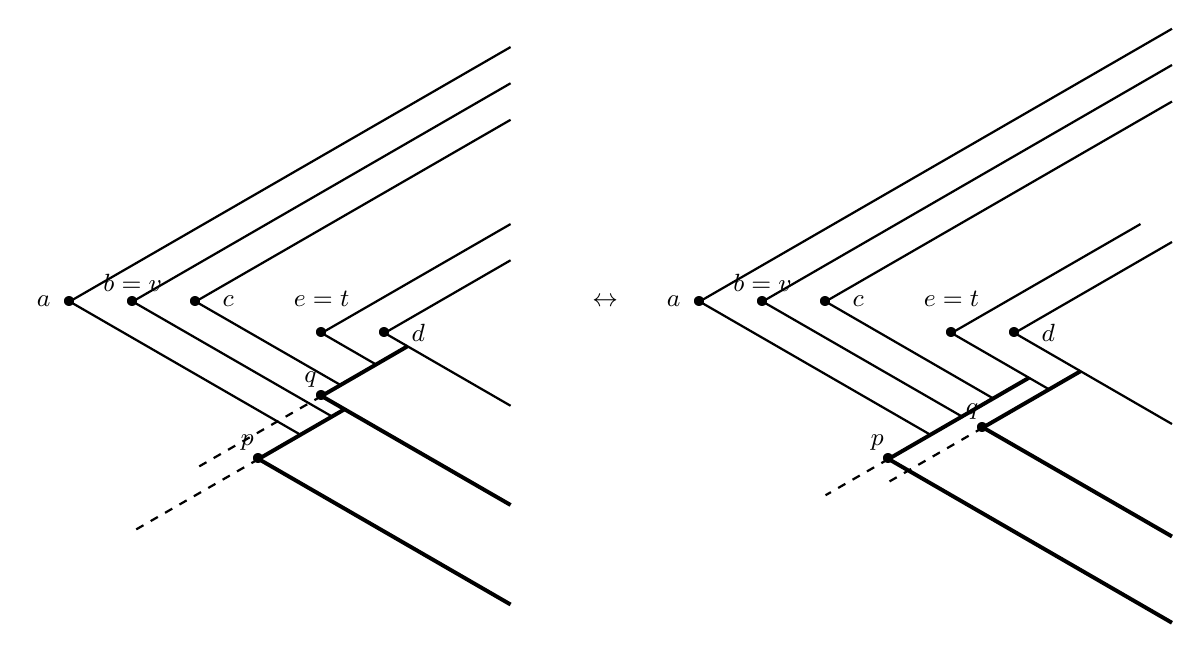
\begin{tikzpicture}[thick, scale=0.4]
        \node[label={[label distance = -3mm]160:$p$}] at
            (6.00, 0.00) {\textbullet};
        \node[label={[label distance = -3mm]160:$q$}] at
            (8.00, 2.00) {\textbullet};
        \node[label={[label distance = -1mm]180:$a$}] at
            (0.00, 5.00) {\textbullet};
        \node[label={[label distance = -2mm]90:$b = v$}] at
            (2.00, 5.00) {\textbullet};
        \node[label={[label distance = 0mm]0:$c$}] at
            (4.00, 5.00) {\textbullet};
        \node[label={[label distance = 0mm]0:$d$}] at
            (10.00, 4.00) {\textbullet};
        \node[label={[label distance = 0mm]90:$e = t$}] at
            (8.00, 4.00) {\textbullet};

        % d cone
        \draw (10.00, 4.00) -- (14.00, 1.69);
        \draw (10.00, 4.00) -- (14.00, 6.31);
        % q cone
        \draw[dashed] (8.00, 2.00) -- (4.00, -0.30);
        \draw[line width = 0.5mm] (8.00, 2.00) -- (14.00, -1.46);
        \draw[line width = 0.5mm] (8.00, 2.00) -- (10.73, 3.58);
        % e cone
        \draw (8.00, 4.00) -- (9.73, 3.00);
        \draw (8.00, 4.00) -- (14.00, 7.46);
        % p cone
        \draw[dashed] (6.00, 0.00) -- (2.00, -2.30);
        \draw[line width = 0.5mm] (6.00, 0.00) -- (14.00, -4.62);
        \draw[line width = 0.5mm] (6.00, 0.00) -- (8.73, 1.58);
        % c cone
        \draw (4.00, 5.00) -- (8.60, 2.35);
        \draw (4.00, 5.00) -- (14.00, 10.77);
        % b cone
        \draw (2.00, 5.00) -- (8.33, 1.35);
        \draw (2.00, 5.00) -- (14.00, 11.93);
        % a cone
        \draw (0.00, 5.00) -- (7.33, 0.77);
        \draw (0.00, 5.00) -- (14.00, 13.08);

        \node at (17, 5) {$ \leftrightarrow$};

        \node[label={[label distance = -3mm]160:$p$}] at
            (26.00, 0.00) {\textbullet};
        \node[label={[label distance = -3mm]160:$q$}] at
            (29.00, 1.00) {\textbullet};
        \node[label={[label distance = -1mm]180:$a$}] at
            (20.00, 5.00) {\textbullet};
        \node[label={[label distance = -2mm]90:$b = v$}] at
            (22.00, 5.00) {\textbullet};
        \node[label={[label distance = 0mm]0:$c$}] at
            (24.00, 5.00) {\textbullet};
        \node[label={[label distance = 0mm]0:$d$}] at
            (30.00, 4.00) {\textbullet};
        \node[label={[label distance = 0mm]90:$e = t$}] at
            (28.00, 4.00) {\textbullet};

        % d cone
        \draw (30.00, 4.00) -- (35.00, 1.11);
        \draw (30.00, 4.00) -- (35.00, 6.89);
        % q cone
        \draw[dashed] (29.00, 1.00) -- (26.00, -0.73);
        \draw[line width = 0.5mm] (29.00, 1.00) -- (35.00, -2.46);
        \draw[line width = 0.5mm] (29.00, 1.00) -- (32.10, 2.79);
        % e cone
        \draw (28.00, 4.00) -- (31.10, 2.21);
        \draw (28.00, 4.00) -- (34.00, 7.46);
        % p cone
        \draw[dashed] (26.00, 0.00) -- (24.00, -1.15);
        \draw[line width = 0.5mm] (26.00, 0.00) -- (35.00, -5.20);
        \draw[line width = 0.5mm] (26.00, 0.00) -- (30.46, 2.58);
        % c cone
        \draw (24.00, 5.00) -- (29.33, 1.92);
        \draw (24.00, 5.00) -- (35.00, 11.35);
        % b cone
        \draw (22.00, 5.00) -- (28.33, 1.35);
        \draw (22.00, 5.00) -- (35.00, 12.51);
        % a cone
        \draw (20.00, 5.00) -- (27.33, 0.77);
        \draw (20.00, 5.00) -- (35.00, 13.66);
    \end{tikzpicture}
    \caption{Da esquerda para direita, o caso em que
    $p$ está em $\Hits_{up}(q)$, ou seja, $q$ está
    entrando em $\Dom(p)$. Da direita para esquerda,
    o caso em que $q$ está em $\Cands(p)$, saindo
    de $\Dom(p)$.}
    \label{fig:parcinetico:eventodown}
\end{figure}

\begin{figure}[h]
    \centering
    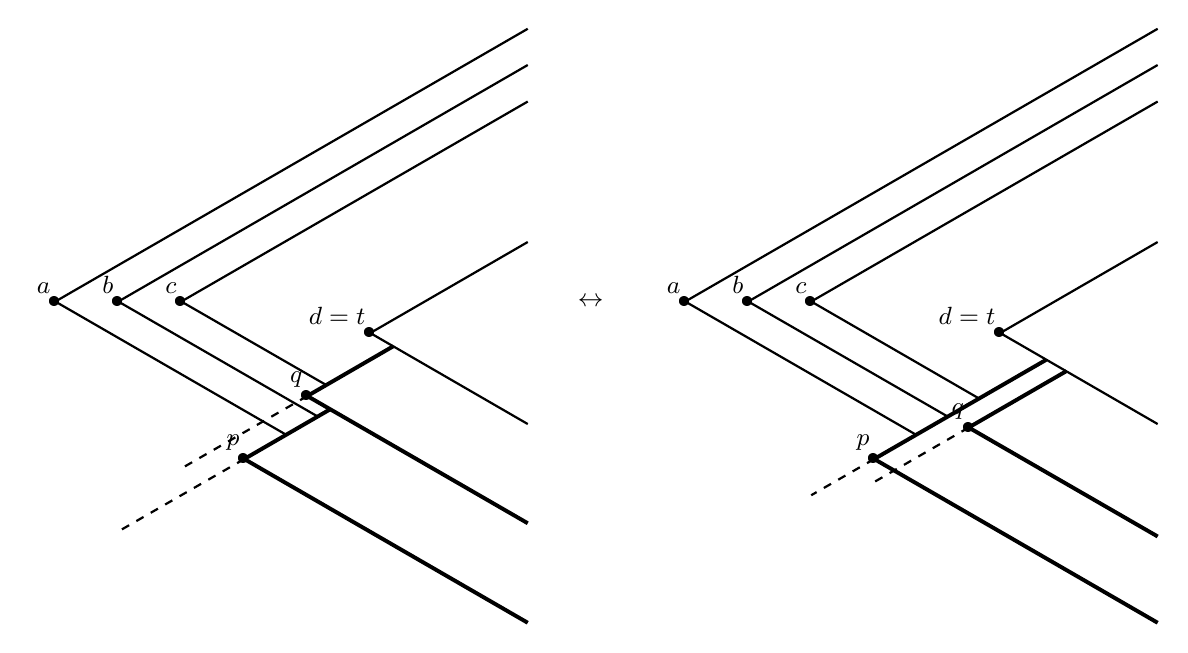
\begin{tikzpicture}[thick, scale=0.4]
        \node[label={[label distance = -3mm]160:$p$}] at
            (6.00, 0.00) {\textbullet};
        \node[label={[label distance = -3mm]160:$q$}] at
            (8.00, 2.00) {\textbullet};
        \node[label={[label distance = -3mm]160:$a$}] at
            (0.00, 5.00) {\textbullet};
        \node[label={[label distance = -3mm]160:$b$}] at
            (2.00, 5.00) {\textbullet};
        \node[label={[label distance = -3mm]160:$c$}] at
            (4.00, 5.00) {\textbullet};
        \node[label={[label distance = -3mm]160:$d = t$}] at
            (10.00, 4.00) {\textbullet};

        % d cone
        \draw (10.00, 4.00) -- (15.00, 1.11);
        \draw (10.00, 4.00) -- (15.00, 6.89);
        % q cone
        \draw[dashed] (8.00, 2.00) -- (4.00, -0.30);
        \draw[line width = 0.5mm] (8.00, 2.00) -- (15.00, -2.04);
        \draw[line width = 0.5mm] (8.00, 2.00) -- (10.73, 3.58);
        % p cone
        \draw[dashed] (6.00, 0.00) -- (2.00, -2.30);
        \draw[line width = 0.5mm] (6.00, 0.00) -- (15.00, -5.20);
        \draw[line width = 0.5mm] (6.00, 0.00) -- (8.73, 1.58);
        % c cone
        \draw (4.00, 5.00) -- (8.60, 2.35);
        \draw (4.00, 5.00) -- (15.00, 11.35);
        % b cone
        \draw (2.00, 5.00) -- (8.33, 1.35);
        \draw (2.00, 5.00) -- (15.00, 12.51);
        % a cone
        \draw (0.00, 5.00) -- (7.33, 0.77);
        \draw (0.00, 5.00) -- (15.00, 13.66);

        \node at (17, 5) {$ \leftrightarrow$};

        \node[label={[label distance = -3mm]160:$p$}] at
            (26.00, 0.00) {\textbullet};
        \node[label={[label distance = -3mm]160:$q$}] at
            (29.00, 1.00) {\textbullet};
        \node[label={[label distance = -3mm]160:$a$}] at
            (20.00, 5.00) {\textbullet};
        \node[label={[label distance = -3mm]160:$b$}] at
            (22.00, 5.00) {\textbullet};
        \node[label={[label distance = -3mm]160:$c$}] at
            (24.00, 5.00) {\textbullet};
        \node[label={[label distance = -3mm]160:$d = t$}] at
            (30.00, 4.00) {\textbullet};

        % d cone
        \draw (30.00, 4.00) -- (35.00, 1.11);
        \draw (30.00, 4.00) -- (35.00, 6.89);
        % q cone
        \draw[dashed] (29.00, 1.00) -- (26.00, -0.73);
        \draw[line width = 0.5mm] (29.00, 1.00) -- (35.00, -2.46);
        \draw[line width = 0.5mm] (29.00, 1.00) -- (32.10, 2.79);
        % p cone
        \draw[dashed] (26.00, 0.00) -- (24.00, -1.15);
        \draw[line width = 0.5mm] (26.00, 0.00) -- (35.00, -5.20);
        \draw[line width = 0.5mm] (26.00, 0.00) -- (31.46, 3.15);
        % c cone
        \draw (24.00, 5.00) -- (29.33, 1.92);
        \draw (24.00, 5.00) -- (35.00, 11.35);
        % b cone
        \draw (22.00, 5.00) -- (28.33, 1.35);
        \draw (22.00, 5.00) -- (35.00, 12.51);
        % a cone
        \draw (20.00, 5.00) -- (27.33, 0.77);
        \draw (20.00, 5.00) -- (35.00, 13.66);
    \end{tikzpicture}
    \caption{Da direita para esquerda, $p$, que estava em $\Hits_{up}(q)$
    foi transferido para $\Hits_{up}(t)$ e todos os elementos em
    $\Hits_{low}(q)$ foram transferidos para $\Hits_{low}(p)$. Da esquerda
    para direita, $p$, que estava em $\Hits_{up}(t)$, foi transferido para
    $\Hits_{up}(q)$ e os pontos à direita de $v$ em $\Hits_{low}(p)$ foram
    transferidos para $\Hits_{low}(q)$.}
    \label{fig:parcinetico:eventodowntnaoexiste}
\end{figure}

\FloatBarrier

\subsection{Análise de desempenho}\label{subsec:par:analise-de-desempenho}

As análises de desempenho aqui foram extraídas de~\cite{eduardo}.

A estrutura de dados cinética para manter um par de pontos mais próximo é uma estrutura
\textit{responsiva}, pois o custo de processar um certificado é $O(\lg{n})$, onde $n$ é o número
de pontos.
O custo de processar um certificado é o custo de realizar as trocas necessárias nas listas
ordenadas, o que consome tempo $O(\lg{n})$.
Além disso também há o custo de corrigir as árvores $\Cands$, $\Hits_{low}$, $\Hits_{up}$, o
torneio e os certificados associados.
Mas, essas operações são realizadas em sequência, consumindo um custo também de $O(\lg{n})$.

A estrutura é \textit{eficiente}, pois a razão entre o total de eventos e os eventos
\textit{externos}, isto é, as trocas de par mais próximo, de acordo com~\cite{eduardo}, é
$O(\epsilon \lg{n})$, resultando em uma estrutura eficiente.

A estrutura é \textit{compacta}, pois teremos $O(n)$ certificados na fila de prioridades
associados a mudanças nas listas ordenadas e $O(n)$ certificados do torneio cinético, resultando
em $O(n)$ certificados na fila com prioridades num determinado instante.

A estrutura é \textit{local}, pois um ponto pode estar envolvido em até seis certificados das
listas ordenadas, sendo dois para cada uma das ordenações, e pode estar envolvido em até
$O(\lg{n})$ certificados no torneio.
